\documentclass[oneside]{htwg-report}

% Use german umlaute
\usepackage{german,ngerman}
\usepackage[T1]{fontenc}
\usepackage[utf8]{inputenc}
\usepackage[ngerman]{babel}
\usepackage[autostyle=true,german=quotes]{csquotes}

%\usepackage[table]{xcolor}\usepackage{float}
%\usepackage{xcolor,colortbl}

\addbibresource{./bib/report.bib}

\begin{document}

\pagenumbering{gobble}

%% 'reporttype' add background elements to the cover / front page
%% possible values are:
%% bachelor	--> B S C
%% master	--> M S C
%% other		--> none
\reporttype{master}

\reporttypetext{Teamproject (Master 3. semester)}

\newcommand{\verfasserA}{Simon Christofzik}
\newcommand{\verfasserB}{Paul Sutter}
\newcommand{\verfasserC}{Till Reitlinger}
\newcommand{\thema}{DeepRain: Rain forecast with neural networks and the visualization of these in an App}
\newcommand{\hoschschule}{HTWG Konstanz - University of Applied Sciences}
\newcommand{\institut}{HTWG Konstanz - Institute for Optical Systems}
\newcommand{\prueferA}{Prof. Dr. Oliver Dürr}


\title[Teamprojektthema]{\thema}

\doclocation{Konstanz}
\docdate{10. September 2020}

\makecover[]

\chapter*{Extended Abstract}

\begin{center}
	\begingroup
	\renewcommand*{\arraystretch}{1}
	\rowcolors{2}{white}{white}
	{\makeatletter	
		\begin{tabular}{p{3.2cm}p{9.6cm}}
			Topic: & \thema \\
			& \\
			Team members: & \verfasserA, \verfasserB, \verfasserC \\
			& \\
			Advisor: & \hoschschule \newline \institut \newline \prueferA \\
			& \\
		\end{tabular}
		
		\makeatother}
	\endgroup
\end{center}

\bigskip

In this Paper we try to predict precipitation for a range of 35 minutes in an area around Constance.
Therefore we are using machine learning techniques and train a UNet on radar data images. 
Here we present the result of precipitation prediction as well with regression as with classification. 
Both approaches provide good results. Source code and full length documentation in german can be found at GitHub: \url{https://github.com/thgnaedi/DeepRain}.


\printbibliography[title={References}, heading=subbibliography]


\twocolumn
\section*{Introduction}

\begin{sloppypar}
\tolerance 9999
Even today, rain forecasts are still very computationally complex and relatively inaccurate. 
Therefore, it may make sense to make such predictions with the help of neural networks. 
These do not require as much computing power and can recognize a pattern in the often chaotic data even without complex physical models.
\end{sloppypar}

\section*{Data}
We are using radar data from the Climate Data Center of the DWD\footnote{\url{https://www.dwd.de/DE/klimaumwelt/cdc/cdc_node.html}}. There are radar images from the years 2004 until 2017.
This data has to be downloaded and converted to png, this is done by our crawler\footnote{\url{https://github.com/thgnaedi/DeepRain/tree/master/DWD_Crawler}} and converter\footnote{\url{https://github.com/thgnaedi/DeepRain/blob/master/Data/DWDtoPngScript.py}}.
The rainfall images then are tailored and scaled. Unattractive images are then rejected, and only interesting images are used for the training.
The resulting images are grayscale PNG files. As network input five temporally consecutive of them are combined to a 3D tensor. The label consists of seven of them.

\section*{Data preprocessing}
To predict precipitation either with regression or classification we are using a UNet.
This Architecture is a convolutional neural network that was at first developed for biomedical image segmentation.
A UNet is a set of convulution layers, combined with an downsampling part, such as pooling layers, and later with upsampling parts like deconvolution layers.

\begin{figure}[ht]
\centering
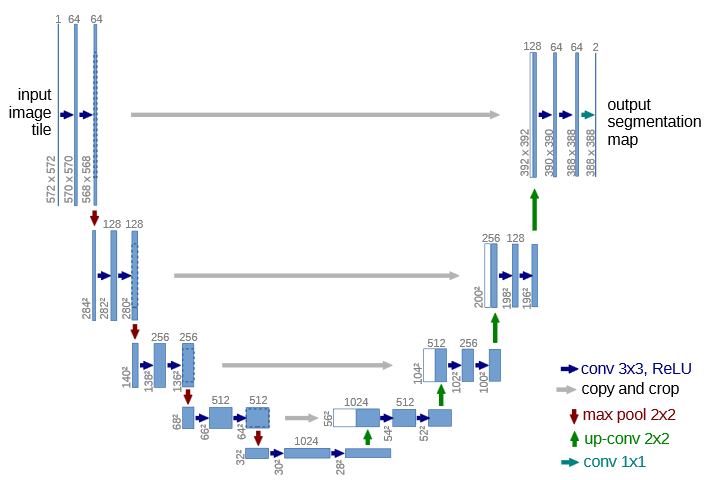
\includegraphics[width=0.8\linewidth]{../pics/UNet_Biomedical}
\caption{The image is taken from the university of Freiburg~\cite{ronneberger2015u}}
\end{figure}

\begin{sloppypar}
\tolerance 9999
\noindent The input images have a shape of 64x64 pixels. They are pooled until the shape reaches a minimum of 8x8 features. Then they are upsampled and concatenated with the downsampling part.
This yields into an u-shaped architecture with crosslinks and is the reason for its name.
\end{sloppypar}

\section*{DeepRain Application}
First approache is to predict the complete radar image. For this regression we use the MSE as lossfunction. The input layer takes the five incoming timesteps and transfers it into a 7 timestep prediction wich reaches up to 35 minutes into the future.
Our network is trained on the radar data from 2005 till 2017. As validation set we use the images from 2004. further information can be found in our full project description\footnote{\url{https://github.com/thgnaedi/DeepRain/blob/master/Docs/Langdokumentation.pdf}}.
The result of this task is shown in the following graphics.

\begin{figure}[ht]
    \centering
    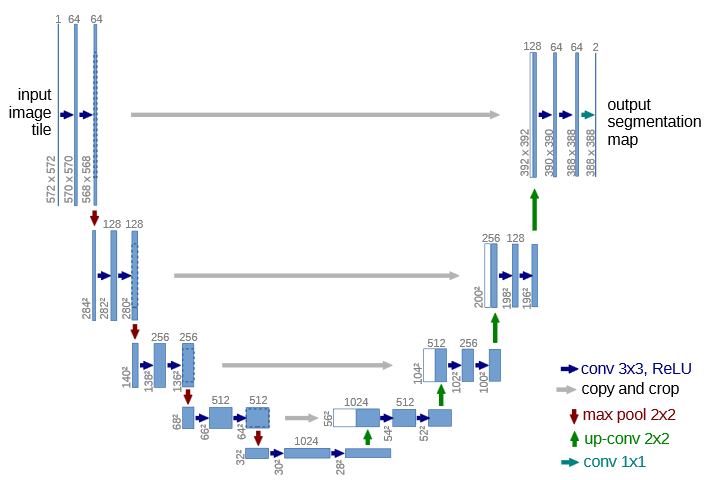
\includegraphics[width=0.8\linewidth]{../pics/UNet_Biomedical}
    \caption{The image is taken from the university of Freiburg~\cite{ronneberger2015u}}
\end{figure}


\begin{figure}[ht]
    \centering
    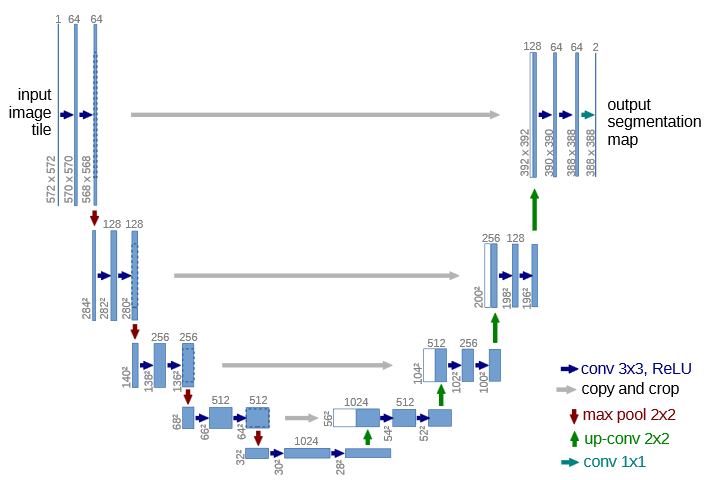
\includegraphics[width=0.8\linewidth]{../pics/UNet_Biomedical}
    \caption{The image is taken from the university of Freiburg~\cite{ronneberger2015u}}
\end{figure}

The predicted values are very close to the label for a difference of only 5 minutes to the input data. The further the time progresses, the worse the prediction becomes.
In the last image it looks like the resolution of the output has been drastically decreased compared to the first output. 
In fact the resolution is the same we can say that this is an indication of uncertainty in the network.
Over time, the movement of the rainfall is well predicted. Even the tiny spot in the top left of images can be predicted.
Even if the area of rainfall increases much faster than in the labels, the center is still well predicted and close to the center of the label.

\section*{Pipeline}
The second approach is to predict the precipitation by classification. Here we try to classify into either three classes (no rain, rain, heavy rain) or two classes (no rain, rain) for each pixel.
Therefore the Unets output is modified to three classes per pixel and an additional softmax layer at the output to provide propabilities. The labels are generated by a threshold for each class.

\begin{figure}[ht]
    \centering
    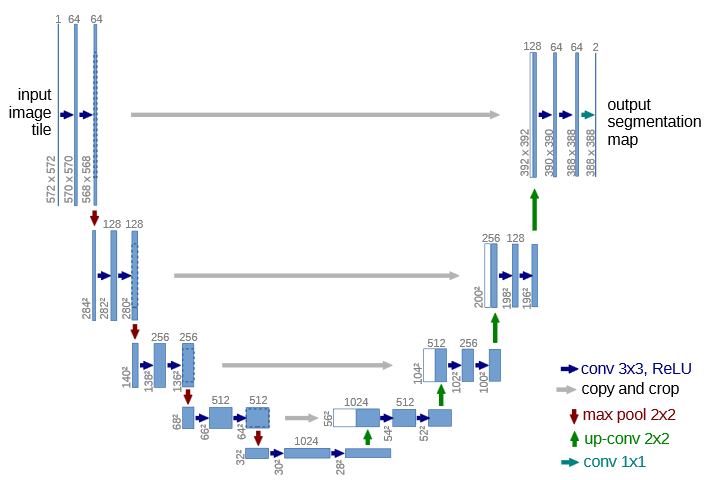
\includegraphics[width=0.8\linewidth]{../pics/UNet_Biomedical}
    \caption{The image is taken from the university of Freiburg~\cite{ronneberger2015u}}
\end{figure}


The gray spots can be rainfall or not depending on the propability of the other two classes. The right image (difference) shows us the absolute difference between the prediction and the label.
Here we can see that the big black spots (no difference between prediction and label) are at the no rainfall labels.
The network has a high accuracy by predicting rainfree pixels. This can be shown in the follwing ROC-image. 
By evaluating the confusion matrix for three class classification, you can recognize that the last class (heavy rainfall) is higly undersampled. 
There are much more rainfall pixels and even more no rainfall pixels in the dataset. To increase the the performance we tried over and undersampling, but both techniques didnt work well for our scenario.
Finally we changed the problem to a two clas classification with a threshold of 0, so the classes are 'no rainfall' and 'rainfall'.

The ROC-curve in figure~\ref{fig:roc} shows how well the two classes rain and no rain can be separated and predicted independent of the number of elements per class.

\begin{figure}[ht]
    \centering
    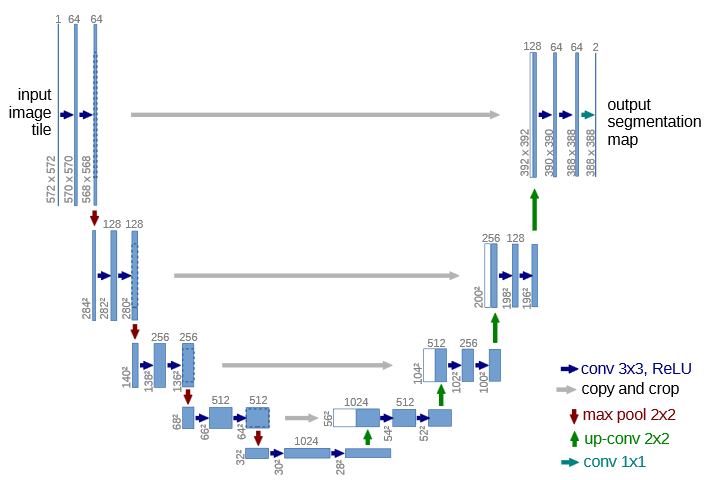
\includegraphics[width=0.8\linewidth]{../pics/UNet_Biomedical}
    \caption{The image is taken from the university of Freiburg~\cite{ronneberger2015u}}
\end{figure}

\section*{Conclusion and Future Work}
In summary, this paper argued that short term precipitation prediction can be done by only observing radar data and without any other source of information.
The accuracy could still be improved as well at the regression, were another lossfunction may could help, as at the classification were the 'rainfall' class is still undersampled and worse accurate than the 'no rain' class.

\end{document}

